% --------------------------------------------------------------
% This is all preamble stuff that you don't have to worry about.
% Head down to where it says "Start here"
% --------------------------------------------------------------
 
\documentclass[12pt]{article}
 
\usepackage[margin=1in]{geometry} 
\usepackage{amsmath,amsthm,amssymb}
\usepackage{listings}
\usepackage{graphicx}

\lstset{
basicstyle=\small\ttfamily,
columns=flexible,
breaklines=true
}
 
\newcommand{\N}{\mathbb{N}}
\newcommand{\Z}{\mathbb{Z}}
 
\newenvironment{theorem}[2][Theorem]{\begin{trivlist}
\item[\hskip \labelsep {\bfseries #1}\hskip \labelsep {\bfseries #2.}]}{\end{trivlist}}
\newenvironment{lemma}[2][Lemma]{\begin{trivlist}
\item[\hskip \labelsep {\bfseries #1}\hskip \labelsep {\bfseries #2.}]}{\end{trivlist}}
\newenvironment{exercise}[2][Exercise]{\begin{trivlist}
\item[\hskip \labelsep {\bfseries #1}\hskip \labelsep {\bfseries #2.}]}{\end{trivlist}}
\newenvironment{problem}[2][Problem]{\begin{trivlist}
\item[\hskip \labelsep {\bfseries #1}\hskip \labelsep {\bfseries #2.}]}{\end{trivlist}}
\newenvironment{question}[2][Question]{\begin{trivlist}
\item[\hskip \labelsep {\bfseries #1}\hskip \labelsep {\bfseries #2.}]}{\end{trivlist}}
\newenvironment{corollary}[2][Corollary]{\begin{trivlist}
\item[\hskip \labelsep {\bfseries #1}\hskip \labelsep {\bfseries #2.}]}{\end{trivlist}}

\newenvironment{solution}{\begin{proof}[Solution]}{\end{proof}}
 
\begin{document}
 
% --------------------------------------------------------------
%                         Start here
% --------------------------------------------------------------
 
\title{Assignment 1: Breaking 6-Round Weak DES}
\author{Rishit D, CS21BTECH11053\\ %replace with your name
Topics in Cryptanalysis} %if necessary, replace with your course title


\maketitle

\section{Introduction}
This report demonstrates a simplified version of the 6-Round DES differential cryptanalysis attack shown in \cite{bsmv}. The attack is performed on a weakened set of S-boxes for each round in the cipher. This attack again invokes the use of \emph{characteristics} with high probability of giving us desired intermediate XOR differences. This, as we shall see, allows us to peel the last layer of the cipher and recover most of the final round subkey.

We remind the reader that borrow the following notation from \cite{bsmv}:
\begin{itemize}
  \item A \emph{characteristic} $\Omega$ is a tuple $(\langle L,R \rangle, \Lambda, \langle l,r \rangle)$ where $\langle L,R \rangle$ is the plaintext XOR difference, $\langle l,r \rangle$ is the ciphertext XOR difference and $\Lambda$ is an another tuple of the form $(\langle a,A \rangle, \langle b,B \rangle, \langle c,C \rangle, \dots)$ where $a,b,c,\dots$ are the input XOR differences to the Fiestel function of each round and $A,B,C,\dots$ are the corresponding output XOR differences to these Fiestel functions.

  \item The \emph{probability} of a characteristic $\Omega$ is denoted by $p^{\Omega}$ and is the product of the probabilities of the individual round characteristics in $\Lambda$.

  \item The \emph{signal-to-noise ratio} of a counting scheme is defined as the ratio of \emph{right pairs} to the \emph{average count} in each counter, where a \emph{right pair} is a pair of plaintexts that satisfy the characteristic at each round. A higher signal-to-noise ration ensures that one can distinguish an accurate counter from all other noisy counters. Mathematically, one can obtain the signal-to-noise ratio as:
    \begin{align*}
      \text{S/R} = \frac{p^{\Omega} \cdot 2^k}{\alpha \cdot \beta}
    \end{align*}
    where $k$ is the number of bits we are searching for, $\alpha$ is the average count per counted pair across all counters and $\beta$ is the ratio of counted pairs to all pairs.
\end{itemize}

\section{Weakness of S-Boxes}
The S-Boxes in the DES cipher are the only non-linear components in the cipher and thereby providing the diffusion required for a secure cipher. Some of the key properties of the S-Boxes include:
\begin{itemize}
  \item The S-Boxes are non-linear and non-affine.
  \item A change in a single bit in the input to the S-Box results in a change in \emph{atleast} two bits in the output.
\end{itemize}

However, the given S-Boxes are weak as there are multiple instances where a single change in the input results in a single change in the output. This is a significant weakness as it allows us to observe multiple S-Boxes and break more bits of the sub-key as we shall see in the following sections.

\section{Constructing the Characteristics}
In the original attack, we utilize two 3-round characteristics to obtain the 42 bits of the subkey for the final round of the cipher. We also want these characteristics to have high probabilities (which empirically can be seen to bounded by $\frac{1}{4}$). The characteristic is shown in the following figure \ref{fig:char1}.

\begin{figure}[!h]
  \centering
  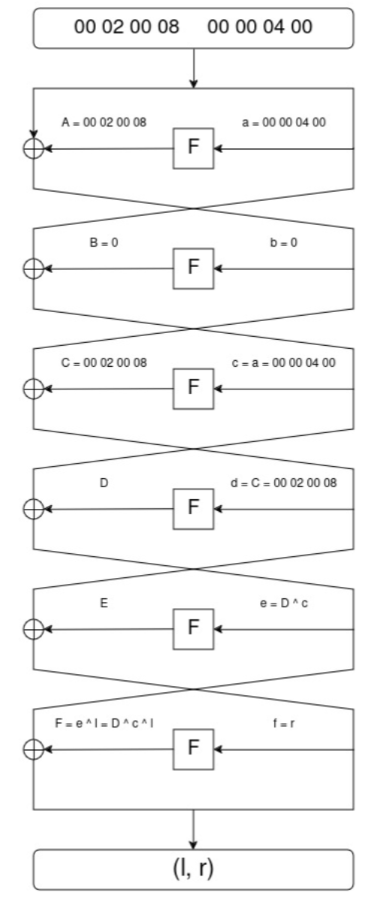
\includegraphics[width=0.4\textwidth]{char1.png}
  \caption{The 3-round characteristic used in the original attack}
  \label{fig:char1}
\end{figure}

\begin{figure}[!h]
  \centering
  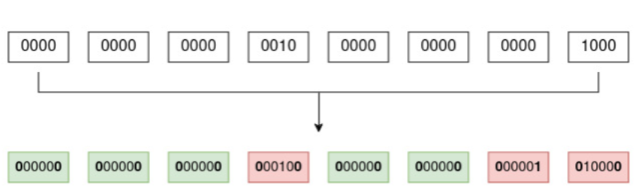
\includegraphics[width=0.8\textwidth]{char1_exp.png}
  \caption{The expansion of $d$ affecting $D$ in the original attack}
\label{fig:exp1}
\end{figure}

This characteristic has the probability of $\frac{1}{16}$ as the first and third round each have a probability of $\frac{1}{4}$ each. We also note how the expansion of $d$ affects $D$ in the figure \ref{fig:exp1}. We can observe that the two ones in $d$ upon expansion results in three S-Boxes with a single change in the output. As a result only, $5$ of the S-Boxes (resulting in $D$) have no change. This allows us to find $30$ subkey bits in the final round via the relation:
\begin{align*}
  F = e \oplus l = D \oplus c \oplus l
\end{align*}
Since $c$ and $l$ are entirely known (along with $30$ bits of $D$), we can compute $30$ bits of the final round subkey$k_6$.

In our case, we have weakened S-Boxes which allows us to exploit even more S-Boxes. Upon analysis of S-Box Differential tables, we see certain instances where a single change in the input results in a single change or no change in the output. One can extract these entries easily by masking the columns and rows with indices as powers of $2$.

Note that (given sufficiently high probability of such transformations), we would like to ideally use a characteristic that gives us no change. This allows us directly obtain $k_6$ without any further analysis/brute-force. Unfortunately, no such instance exists as these input bits are \emph{expanded} to other S-Boxes, making them have atleast one change.

Consequently, we look at S-Boxes that exactly change one bit of the output and find that the following characteristic is ideal for our purposes as shown in figure \ref{fig:char2}.

\begin{figure}[!h]
  \centering
  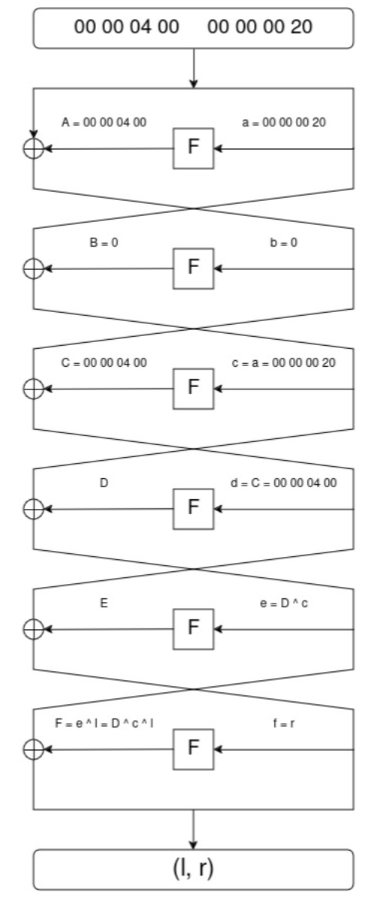
\includegraphics[width=0.4\textwidth]{char2.png}
  \caption{The 3-round characteristic used in the weakened attack}
  \label{fig:char2}
\end{figure}

We also note that the expansion only results in uncertainty of the $6^{th}$ S-Box, thereby allowing us to find $42$ bits of the final round subkey $k_6$, leaving only $6$ bits to be brute-forced (apart from the $8$ bits not present in $k_6$). We also choose this characteristic due to its high probability of $\frac{3}{8}$ per round, giving us a total probability of $\frac{9}{64} > \frac{1}{16}$.

\begin{figure}[!h]
  \centering
  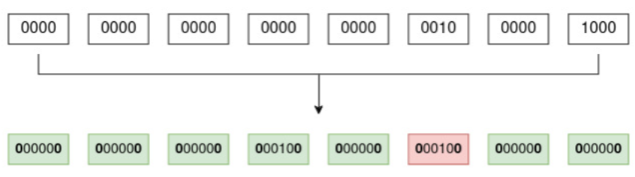
\includegraphics[width=0.8\textwidth]{char2_exp.png}
  \caption{The expansion of $d$ affecting $D$ in the weakened attack}
  \label{fig:exp2}
\end{figure}

One can analyse the above differentials via \texttt{s\_box\_diff.py} which loads S-box differential tables and also produces specific entries that might be ideal for building characteristics.

\section{Signal-to-Noise Ratio}
For this scheme, our signal-to-noise ratio is given by:
\begin{align*}
  \text{S/R} = \frac{\frac{9}{64} \cdot 2^{42}}{4^7} \approx 2^{25.17}
\end{align*}
Our average count $\alpha$ is $4^7$ as we have $7$ S-Boxes that we are counting pairs for and the number of counters is $2^{42}$ as we are searching for $42$ bits of the subkey.

Note that this is a very high signal-to-noise ratio as compared to the original attack (with $2^{16}$). Consquently, we will significantly reduce the number of pairs ($\approx 120$) from the original attack.

\section{Overview of the Attack}
The attack can be executed by \texttt{final\_key.py} which generates the final key by applying the above characteristic and peeling the last round of the cipher. We then brute-force the remaining $14$ bits of the master key to obtain the total master key.

\subsection{Creating Pairs}
We first create pairs of plaintexts that satisfy the input XOR difference of the characteristic. Note that this need not be a \emph{right pair} as this cannot always guarantee that the characteristic holds (since $\Omega$ is probabilistic). We then encrypt these pairs and store the ciphertexts as a list of tuples. We also ensure that we first apply the inverse of the initial permutation to the plaintexts and the final permutation to the ciphertexts, in order to ensure that characteristic positions are consistent.

We now need to construct the possible keys for each $S-Box$ for each plaintext-ciphertext pair. Using the relation $F = D \oplus c \oplus l$, we can obtain the output XOR of the Fiestel function (of the last round) for each pair. We also know each of the inputs to the Fiestel function through $f = r$.

We peel of the expansion and permutation layers of the final Fiestel function by applying the inverse of the mixing permutation on $F$ and expanding each of the inputs $f$ using the expansion permutation. One can now brute-force over all $64$ keys for each $S-Box$ to obtain a keymask for each $S-Box$.

\subsection{Counting Pairs: MAX-CLIQUE}
One can naively count pairs using $2^{42}$ counters which is highly infeasible. Instead, we form edges between plaintext pairs that have commonly suggested keys (ie) non-zero intersection of key-masks. The biggest clique in this graph ideally contains a common key for each S-Box (ie) a power-of-two keymask. We utilize a standard recursive approach to find the maximum clique in the graph. We also ignore pairs that have a $0$ keymask as they represent \emph{wrong pairs}. Once we have the vertices in the maximum clique, all the keymasks are intersected to obtain the final keymask for each S-Box.

\subsection{Brute-Forcing the Master Key}
We first use the key-scheduling algorithm to identify the indices of the original key being used in the last round subkey $k_6$. We then create a template for the master key by setting the known bits of the master key to the known bits of $k_6$ via the generated key-schedule. We then brute-force the unknown bits (excluding the parity bits) of the master key, compute parity bits and verify if the key is correct over a small set of plaintext-ciphertext pairs.

\section{Results}
Our final obtained key is \texttt{0101011101000101011011101000010110111010101000101011010101001100}. The total number of pairs used for the counting scheme was $85$ pairs (ie) $170$ ciphertexts. We also utilized $5$ more ciphertexts for brute-forcing the master key.

\bibliographystyle{plain}
\bibliography{references}

\end{document}

